\documentclass[UTF8]{ctexart}
\usepackage{ctex}
\usepackage{geometry}
\usepackage{enumitem}
\usepackage{indentfirst}
\usepackage{color}
\usepackage{fancyhdr}
\usepackage{amsmath}
\usepackage{graphicx}
\usepackage{amssymb}
\usepackage{tikz}
\usepackage{cases}
\usepackage{array}
\usepackage{pgfplots}
\usepackage{tkz-euclide}
\usepackage{mathrsfs}
% 设置纸张和页边距——A4
\geometry{papersize={21cm,29.7cm}}
\geometry{left=3.18cm,right=3.18cm,top=2.54cm,bottom=2.54cm}

% 一级标题靠左
\CTEXsetup[format={\Large\bfseries}]{section}

% 去除页眉
\pagestyle{plain}

%设置段间距
\addtolength{\parskip}{.4em}
%%设置行间距
%\usepackage{setspace}
%\setstretch{2.5}

% 开始文档内容
\begin{document}

\title{信号与系统课程笔记:Lecture 29:系统的状态空间分析}
\author{授课教师:秦雨潇 \\
        笔记记录:曹时成}
\date{2023 年 12 月 20 日(第十六周,周三)}
\maketitle

\section{课程重点梳理}
(1) 一般信号怎么分解为特殊信号  \par
(2) 特殊信号通过系统的变化与性质 \par
(3) 一般信号通过系统的变化与性质 \par
重点内容:傅里叶变换和采样定理 \par

\section{课堂回顾}
谐波信号通过系统 \par
$ f(t)=Ae^{j\omega_0 t}=Acos(\omega_0 t+\varphi_0)\longrightarrow $ \boxed{H(t)} $\longrightarrow | H(\omega_0 )\vert Acos(\omega_0 t+\varphi_0+\angle H(\omega ))$ \par
1. $f(t)/f[k]$ \par
\qquad  $\updownarrow $ \quad  $\updownarrow $ \par
\qquad  s \quad z \par
2.  \par
(1)$H(z)$ \qquad $f[k]\longrightarrow H(z) \longrightarrow ?$ \par
\qquad $H(\omega_0)=H(z)\vert_{z=e^{j\omega_0}}$ \par
(2)$H(s)$ \qquad $f(t)\longrightarrow H(s) \longrightarrow ?$ \par
\qquad $H(\omega_0)=H(s)\vert_{s=j\omega_0}$ \par

\section{基本概念和定义}
状态方程:表示系统状态变量与输入之间的关系的方程。 \par
n阶系统:由n个一阶微分/差分方程组构成。 \par
输出方程:表示系统输入输出和状态变量之间的关系的方程。\par
对于n阶系统,如果有q个输出,则输出方程由q个代数方程组构成。\par
\section{建立系统的状态方程和输出方程}
\subsection{初始状态}
$x_1(0^-),x_2(0^-),\cdots ,x_n(0^-)$ \par
注意:\par
(1)电路中,一般来说,电容的系统状态选择$U_c$ ;电感的系统状态选择$i_l$  \par
(2)系统状态数目是一定的,n阶系统有n个初始状态。但是,状态方程的列法不唯一。 \par
\subsection{状态变量}
状态变量:表示状态随时间变化的一组变量。 \par
\subsection{状态矢量/状态空间}
$[ x_1(0^-),x_2(0^-),\cdots ,x_n(0^-)]^T$ \par
状态空间为状态矢量构成的空间。\par
\subsection{状态方程}
状态方程:假设有n阶和p个输入 \par
$x_1'=a_{11}x_1+a_{12}x_2+\cdots +a_{1n}x_n+b_{11}f_1+\cdots +b_{1p}f_p$ \par
$\vdots $ \par
$x_n'=a_{n1}x_1+a_{n2}x_2+\cdots +a_{nn}x_n+b_{n1}f_1+\cdots +b_{np}f_p$ \par
\begin{equation}
        \left[   
           \begin{matrix}
           x_1'(t) \\
           x_2'(t) \\
           \vdots'(t) \\
           x_n'(t) \\
           \end{matrix}
         \right]
         =  \left[   
           \begin{matrix}
           a_{11} &  a_{12} & \cdots & a_{1n}  \\
           a_{21} &  a_{22} & \cdots & a_{2n}  \\
           \vdots  &  \ddots   & \vdots   \\
           a_{n1} &  a_{n2} & \cdots & a_{nn}  \\
           \end{matrix}
         \right]
         \left[   
          \begin{matrix}
          x_1(t) \\
          x_2(t) \\
          \vdots'(t) \\
          x_n(t) \\
          \end{matrix}
        \right]
        +  \left[   
          \begin{matrix}
          b_{11}  & \cdots & b_{1p}  \\
          b_{21}  & \cdots & b_{2p}  \\
          \vdots  & \ddots& \vdots   \\
          b_{n1} & \cdots & b_{np}  \\
          \end{matrix}
        \right]
        \left[   
          \begin{matrix}
          f_1(t) \\
          \vdots'(t) \\
          f_p(t) \\
          \end{matrix}
        \right]
        \nonumber
       \end{equation}
\begin{equation}
  \dot{\bm{X}} = \bm{AX} + \bm{BF}\triangleq \text{状态方程}
  \nonumber
\end{equation}
\subsection{输出方程}
输出方程:描述系统输入输出和状态之间的代数方程组,假设有q个输出,则: \par
$y_1=c_{11}x_1+c_{12}x_2+\cdots +c_{1n}x_n+d_{11}f_1+\cdots +d_{1p}f_p$ \par
$\vdots $ \par
$y_q=c_{q1}x_1+c_{q2}x_2+\cdots +c_{qn}x_n+d_{n1}f_1+\cdots +d_{qp}f_p$ \par
\begin{equation}
  \dot{\bm{Y}} = \bm{CX} + \bm{DF}\triangleq \text{输出方程}
  \nonumber
\end{equation}

\section{例1}
\begin{figure}[h]
  \centering         %使图片居中放置
  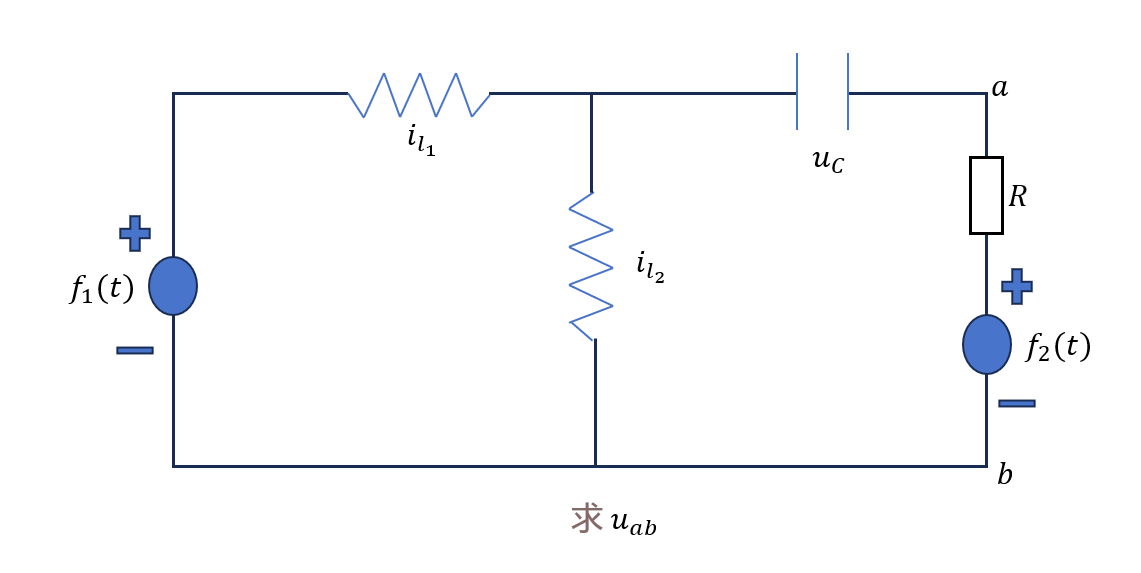
\includegraphics[scale=0.38]{1.png}
\end{figure}
解: \par
状态变量: \par
$x_1=i_{L_1}$ \qquad $x_2=i_{L_2}$ \qquad $x_3=u_{c}$ \par 
电压(Ku):\par
$ x_1'=f_1-x_3-R(x_1-x_2)-f_2=-\frac{R}{L_1} x_1+\frac{R}{L_1} x_2-\frac{1}{L_1} x_3+\frac{1}{L_1} f_1-\frac{1}{L_1} f_2 $\par 
$ x_2'=u_{L_2}=x_3+R(x_1-x_2)+f_2=-\frac{R}{L_2} x_1-\frac{R}{L_2} x_2+\frac{1}{L_2} x_3+\frac{1}{L_2} f_2 $\par
电流(Kcl):\par
$ x_3'=i_{L_1}-i_{L_2}=x_1-x_2=\frac{1}{L} x_1-\frac{1}{L} x_2 $ \par
\begin{equation}
  \left[   
     \begin{matrix}
     x_1'(t) \\
     x_2'(t) \\
     x_3'(t) \\
     \end{matrix}
   \right]
   =  \left[   
     \begin{matrix}
     -\frac{R}{L_1}  &  \frac{R}{L_1} & -\frac{1}{L_1}  \\
     \frac{R}{L_2}  &  -\frac{R}{L_2} & \frac{1}{L_2}  \\
     \frac{1}{c}  &  -\frac{1}{c} & 0  \\
     \end{matrix}
   \right]
  +  \left[   
    \begin{matrix}
    \frac{1}{L_1}  & -\frac{1}{L_1}  \\
    0  & \frac{1}{L_2}  \\
    0  & 0  \\
    \end{matrix}
  \right]
  \left[   
    \begin{matrix}
    f_1 \\
    f_2 \\
    \end{matrix}
  \right]
  \nonumber
 \end{equation}
def:状态空间=状态方程+输出方程 \par
输出:$y_1=u_{L_2},y_2=u_{ab} $ \par
$ y_1=L_2x_2'=R(x_1-x_2)+x3+f_2 $ \par
$ y_2=Ri_R+f_2=R(x_1-x_2)+f_2 $ \par
$\Rightarrow $
\begin{equation}
  \left[   
     \begin{matrix}
     y_1 \\
     y_2 \\
     \end{matrix}
   \right]
   =  \left[   
     \begin{matrix}
     -R  &  R & 1  \\
     R  &  -R & 0  \\
     \end{matrix}
   \right]
   \left[   
    \begin{matrix}
    x_1 \\
    x_2 \\
    x_3 \\
    \end{matrix}
  \right]
  +\left[   
    \begin{matrix}
    0 & 1  \\
    0 & 1  \\
    \end{matrix}
  \right]
  \left[   
    \begin{matrix}
    f_1 \\
    f_2 \\
    \end{matrix}
  \right]
  \nonumber
 \end{equation}
\end{document}